% I would rather have a bit of space between paragraphs
\setlength{\parskip}{0.5\baselineskip}

% I would like to include the abstract at the top
\begin{quote}
\small
\articleABSTRACT
\end{quote}


\section{Introduction}

\citet{lamichhane2003} described a Bayesian statistical method for
estimating the number and identity of essential genes in a genome from
data that indicates viable mutants. The genome of \emph{Mycobacterium
tuberculosis\/} was mutagenized with a transposon that inserted at
known sites, and a library of viable mutants was characterized. If a
mutant with insertion that disrupted a particular gene was viable,
that gene was indicated to be non-essential. Essential genes are those
for which no disruptive mutation could be viable.

The analysis method, described in further detail in
\citet{blades2002}, sought to estimate the overall proportion of
essential genes, and the probability that a gene was essential. We
assumed a uniform prior distribution on the number of essential genes,
and that genes were equally likely to be essential, and used Markov
chain Monte Carlo to derive the posterior probabilities of genes being
essential.

As part of the ReScience Ten Years Reproducibility Challenge, I sought
to reproduce the analysis in the paper, which I conducted in 2002
while an assistant professor in the Department of Biostatistics at
Johns Hopkins University. The bulk of the data and code were quickly
identified. (I keep collaborative projects in a directory
\verb|~/Projects| and save old projects in compressed form in
\verb|~/Projects/Tar|, and I immediately found
the file \verb|Gyanu.tgz|. Gyanu Lamichhane was first author on the
paper.) However, there were a number of challenges in reconstructing
the analysis steps, and the code used to conduct the computer
simulations underlying Figure~3 of \citet{lamichhane2003} appears
lost; I found only the results and the code to generate the figure.

The method was implemented in a combination of R \citep{R} and C
\citep{C} and assembled as an R package, R/negenes \citep{negenes},
which is available on both
\href{https://github.com/kbroman/negenes}{GitHub} and the
\href{https://cran.r-project.org/package=negenes}{Comprehensive R
  Archive Network (CRAN)}. The software used for the analyses in the
paper are a set of R scripts, along with one Perl script
\citep{Perl} that extracted transposon insertion sites from the \emph{M.
tuberculosis\/} genome.

\section{Challenges}

Talk about the mess that I left myself.

\begin{figure}
\definecolor{offwhite}{RGB}{255,250,240}
\lstset{language=bash,
        basicstyle=\ttfamily\scriptsize,
        frame=single,
        commentstyle=,
        backgroundcolor=\color{offwhite},
        showspaces=false,
        showstringspaces=false
        }

\begin{lstlisting}
class_problems.txt        findTA.pl*        Randomness/
Converge/                 mindGaps.pl*      Rawdata/
crucial_doubleTA.txt      Nov02/            Sept02/
Data/                     Operons/          Sims/
doubleta_hit.txt          R/                TroubleShootingSubClasses.txt
exploreSeq.pl*
\end{lstlisting}

\caption{Project directory for the work}
\end{figure}


\section{Code modifications}

\section{The R/negenes package}

Talk about maintenance and changes of the R package.

Original analysis with R version 1.5.1 (2002-06-17)
latest with R version 3.6.1 (2019-07-05).


\section{Results}

\begin{figure}
\includegraphics[viewport=133 224 464 528, width=0.50\textwidth]{../original/Nov02/R/Figs/fig1.ps}
\hfill
\includegraphics[viewport=133 224 464 528, width=0.50\textwidth]{../reproduction/Figs/fig1.ps}

\caption{Figure 1a in Lamichhane et al. (2003). Original on left. Reproduction on right.}
\end{figure}

\begin{figure}
\includegraphics[viewport=179 299 438 517, width=0.50\textwidth]{../talk/Figs/circlefig.ps}
\hfill
\includegraphics[viewport=179 299 438 517, width=0.50\textwidth]{../reproduction/Figs/circlefig.ps}

\caption{Figure 1b in Lamichhane et al. (2003). Original on left. Reproduction on right.}
\end{figure}

\begin{figure}
\includegraphics[viewport=44 245 525 508, width=0.50\textwidth]{../original/Nov02/R/Figs/fig2.ps}
\hfill
\includegraphics[viewport=44 245 525 508, width=0.50\textwidth]{../reproduction/Figs/fig2.ps}

\caption{Figure 2 in Lamichhane et al. (2003). Original on left. Reproduction on right.}
\end{figure}
